\documentclass[12pt,a4paper,twocolumn]{article}

\usepackage[top=0.8in,bottom=0.8in,right=0.8in,left=0.8in]{geometry}

%for links
\usepackage{hyperref}

%for bilbiography
\usepackage{natbib}

%for images
\usepackage{graphicx}
\usepackage{caption}
\usepackage{subcaption}

\graphicspath{./img/}


\author{Dionisio Perez-Mavrogenis}
\title{Firmware Protection and Attacks Against the ATMega Microcontroller Series}
\date{\today}

\begin{document}
	\maketitle
	
\section*{Abstract}
	Give paper topic, objectives and conclusions reached.
	

\section{Introduction}
	mention abbreviation mcu=microcontroller unit. 
	\subsection{Problem Statement}
	Perhaps need to classify attackers : e.g. home hacker $<<$ (semi-)professional crackers $<<$ funded organisations. also give potential problems(financial and security implications) with stolen software (IP theft etc), firmware tampering etc. Also separate microcontrollers (designed for high security or ordinary use)

	\subsection{Objectives of Paper}
	\begin{itemize}
	\item Review the ATmega series (architecture, applications and security features)\\
	\item Review current attacks against MCUs in general \\
	\item Review Countermeasure to these attacks or how to make them more difficult
	\item Review attacks applicable to the ATmega (give the easiest possible attack applicable)
	\item Describe a way to make the mega more secure
	\item Evaluate if it's worth going the extra mile for security
	\item Have an overview of the paper in the conclusion
	\end{itemize}
	
	Give paper structure at some point.
	

\section{The ATMega MCU Series}
	The ATmega series of MCUs is a popular microcontroller family for a number of reasons, offering a combination of a reasonably powerful MCU at a low price. They offer a variety of clock speeds and memory capacities (with processor speeds of up to 20MHz and up to 256Kb of flash memory) and large operating voltage windows, hence making them both power efficient as well as enabling them to interact with peripherals with different operating voltages\footnote{info here \href{https://www.newbiehack.com/MicrocontrollersAlternativePowerSources.aspx}{https://www.newbiehack.com}}\footnote{taken from:\href{http://www.atmel.com/v2PFResults.aspx}{http://www.atmel.com/v2PFResults.aspx}}.
	
	Furthermore, developing software for an AVR board is very easy, a further incentive to use an AVR over other popular options. In particular, the AVR MCUs benefit from the free \texttt{avr-libc} high-performance C run-time library(optimised for the AVR), the \texttt{avr-gcc} and \texttt{avr-gdb} compiler and debugger(both based on very popular and high quality GNU software tools), the \texttt{avrdude} programming software(or Atmel's proprietary \texttt{AVRStudio}) and \texttt{Simulavr} simulator software. In addition to these community tools, Atmel provides proprietary APIs for interacting with the AVR and the developers can choose from a wide variety of programmer units available for working with the AVR MCUs.
	
	\subsection{AVR Predecessors to the ATmega Series}
	apparently sergei has cracked them already
	maybe talk about support(libraries/tools) here ?? \cite{website:scorobogatov_breaking_copy_protection}
	\subsection{ATMega Architecture and Features}				
By combining an 8-bit RISC CPU with In-System Self-Programmable Flash on a monolithic chip,the Atmel ATmega644 is a powerful microcontroller that provides a highly flexible and cost effective solution to many embedded control applications.The ATmega644 AVR is supported with a full suite of program and system development tools including: C compilers, macro assemblers, program debugger/simulators, in-circuit emulators, and evaluation kits.	

	\subsubsection{Background and General Features}
	The ATmega series of MCUs is a relatively large family of microntroller units. However this paper focuses only on the ATmega644 and ATmega1284, [reasons for focus here]. The only difference between then 1284 and the 644 is that the 1284 has got more memory available and a summary of (some) of the features of the two units is give in Table \ref{table:avr_specs}[\citep{atmega644_manual},\citep{atmega1284_manual}]. 
	
	Both MCUs are an enhanced RISC Harvard architecture 8-bit CPU. Figure \ref{fig:architectures} shows the conceptual difference between a Von Neuman (most modern PCs) and a Harvard architecture, where the key distinction lies in the separation of application code and program data into different memory sections (Harvard) and tasking the CPU with distinguishing between code and data that lives in the same memory region (Von Neuman). The 644/1284 implement a Harvard architecture for both power and computational efficiency, as they are able to access more than one registers simultaneously (due to the physical wiring of the CPU) and hence are able to execute an instruction per cycle as once an instruction is executing the next one is pre-fetched and decoded. Their operating voltages can vary between 1.8V and 5.5V (maximum operating frequency 20 MHz).
	
	\subsubsection{Memory Organisation}
	The 644/1284 are equipped with an EEPROM, flash memory, SRAM, a large number of general purpose registers and a large number of I/O registers (in order to be able to perform I/O) and all memory (including I/O memory mapped images) is linear, i.e. it follows the flat memory model.
	
	The flash memory is separated into two regions, the bootloader section and application code section. The boundary between the two sections can be configured by programming the appropriate fuses, and the page size can also be configured that way as well. Both sections hold code, however code residing in the bootloader section can execute a special instruction (\texttt{SPM}\footnote{SPM = Store Program Code}) which allows the bootloader code to write to \textit{any} section in the flash memory and hence possibly modify itself(designed for purposes such as firmware upgrades). The bootloader code can be triggered by a direct jump from the application section or by programming the reset vector via the reset fuse to point to the appropriate section of the bootloader code. 
	
	The EEPROM is memory for data that needs to persist between reboots of the MCU and hence it is (widely) used to hold configuration variables and other non-temporary preferences the application code (or the bootloader) may need, having an average lifespan is 100,000 write cycles per page. 
	
	The SRAM is volatile storage and is used as the stack and heap for the software (either application code or bootloader code) as well as for storing the Register File (i.e. the 32 GP registers) I/O and Extended I/O Memory. The reserved register locations exist in order to support the use of peripheral units as well as hold program status information (e.g. the Stack Pointer can be found in one of the GP registers).Figure \ref{fig:stack} gives an overview of the SRAM hierarchy, which is slightly different (in terms of region sizes) for the 644 and the 1284 as the 1284 offers more SRAM.
	
	\begin{figure}
		% source : atmel's manuals 
		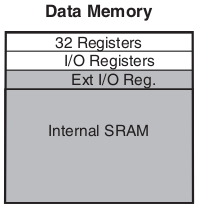
\includegraphics[scale=1]{img/stack.png}
		\caption{SRAM layout for the ATmega 644 and 1284.}
		\label{fig:stack}		
	\end{figure}
	
\begin{figure}
	\begin{subfigure}[b]{0.3\textwidth}
		% source http://www.elec.canterbury.ac.nz/PublicArea/Staff/hof/p10-embed/p10-tutorial/p12.html
		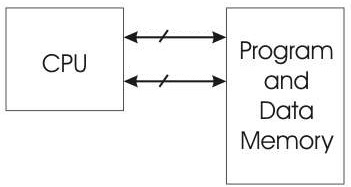
\includegraphics[scale=0.65]{img/von_neuman_arch.jpg}
		\caption{Schematic of a Von Neuman architecture.}
		\label{fig:VN_arch}
	\end{subfigure} \\
	
	\begin{subfigure}[b]{0.3\textwidth}
		% source : http://www.elec.canterbury.ac.nz/PublicArea/Staff/hof/p10-embed/p10-tutorial/p13.html
		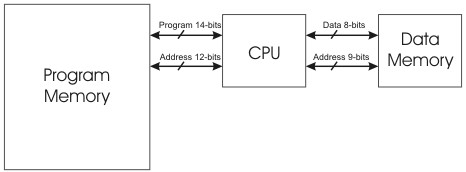
\includegraphics[scale=0.5]{img/harvard_arch.jpeg}
		\caption{Schematic of a Harvard architecture.}
		\label{fig:H_arch}
	\end{subfigure}
	\caption{A comparison of different machine architectures.}
	\label{fig:architectures}
\end{figure}	
		
	\begin{table*}
		\begin{tabular}{| c | p{2cm} | p{1.5cm} | p{3cm} | p{2.8cm} | c | p{1.9cm} |}
		\textbf{Model} & \textbf{EEPROM (Kb)} & \textbf{SRAM (Kb)} & \textbf{Programmable Flash(Kb)} & \textbf{GP Registers} & \textbf{SPI Port} & \textbf{JTAG Interface}\\
		ATmega644 & 2 & 4 & 64 & 32 & Yes & Yes\\
		ATmega1284 & 4 & 16 & 128 & 32 & Yes & Yes \\
		
		
		\end{tabular}
	\caption{Specification overview for the AVR ATmega644 and ATmega<>}
	\label{table:avr_specs}
	\end{table*}
	
	\subsection{ATMega Security Features}
	
	The AVR ATmega644/1284, even though they are not meant to be trusted or secure hardware, posses certain security features. In particular, each board provides six Lock bits (which can be programmed or unprogrammed) and which are responsible for controlling or preventing different memory portions of the board to be modified or read by the other parts (e.g. prevent code executing from the bootloader section to read/write the application code section via the \texttt{SPM} instruction). The prevention however is not permanent, as that would limit the usefulness of the MCU and therefore one has the option to bring these lock bits back to State 1 (i.e. unprogrammed, having no protection scheme enabled) by issuing a Chip Erase command, which has the effect of completely erasing the Flash, EEPROM and Lock bits.
	
	The erasing is performed with the sequence of events presented above and this is important, as one does not want to remove the access protection before removing all sensitive data and hence the Lock bits are set to 1 only after the whole program memory has been erased. Even though the flash memory has an average lifespan of 10,000 write cycles (as well as programming being relatively expensive as an operation) this approach makes sense as the ultimate goal is to preserve the intellectual property on the board rather than the board itself.
	
	\begin{table*}
		\center
		\begin{tabular}{| c | c | c | c |}
			\hline
			\textbf{Lock Bit Byte} & \textbf{Bit Number} & \textbf{Description} & \textbf{Default Value}\\
			\hline \hline
			BLB12 & 5 & Boot Lock Bit & 1\\
			BLB11 & 4 & Boot Lock Bit & 1\\
			BLB02 & 3 & Boot Lock Bit & 1\\
			BLB01 & 2 & Boot Lock Bit & 1\\
			LB2 & 2 & Lock Bit & 1 \\
			LB1 & 1 & Lock Bit & 1 \\
			\hline
		\end{tabular}
		\caption{Security lock bits offered by the ATmega644 and ATmega1284.}
		\label{table:lock_bits}
	\end{table*}
	
Table \ref{table:lock_bits}	 provides an outline of the available Lock bits provided by the ATmega series. The functionality of the BLB1 group is to control access and modification of the bootloader section, group BLB0 bits control access to the application code section and group LB bits are responsible for controlling modifications on the EEPROM and Flash.A detailed explanation of their functionality and how to use them is given in \citep{atmega1284_manual} and \citep{atmega644_manual}.
	
\section{Current Attacks}
	\subsection{Introduction}
	mention attacks may be passive(observing input-$>$output mapping) or active (tamper with the aforementioned mapping in some useful way)
	\subsection{Non-Invasive Attacks}
	\subsection{Semi-Invasive Attacks}
		all memory types are linear( as well as memory mapped IO) - related to memory scanning attacks by glitching and power faults (stop making call or jump instructions)
	\subsection{Invasive Attacks}

	overview of attack categories [each one to the category that it corresponds above]
	\begin{itemize}
		\item microprobing \\
		\item side-channel attacks \\
		\item software attacks (exploit communication protocols or crypto implementation and such) \\
		\item reverse engineering of hardware\\
		\item fault generation (power/clock glitches ) \\
	\end{itemize}
	
	* for each category discuss budget/tools/skillset/time required\\

\section{Countermeasures to known attacks}
	\begin{itemize}
	\item overview of most popular techniques \\
	\item benefits and how they improve the situation/approach the problem
	\item added cost for this investment (in terms of hardware and money, transparency to the developers, runtime overhead etc)\\
	\end{itemize}
	
	perhaps review some popular secure chips ??	
	
	

\section{Securing the mega}
	\subsection{Working attacks against the ATmega}
	\subsection{Motivation}
	\subsection{Current Attack Vectors}
	\subsection{Protective Steps}
		* feasible? 
		* added cost (in terms of \$\$, extra hardware and software implementation penalties/overhead)
	

\section{Evaluation}
	not sure if the subsections are needed here
	\subsection{Attacks and Solutions overview}
	\subsection{Conclusions}
	
	\pagebreak
	\onecolumn
	\bibliographystyle{plain}
	\bibliography{irp_report}	
	
\end{document}
